\documentclass[mingoth,11pt,a4j,uplatex]{jsarticle}
\usepackage[top=20truemm,bottom=20truemm,left=20truemm,right=20truemm]{geometry}
\usepackage{moreverb}
\usepackage{listings,jlisting} %日本語のコメントアウトをする場合jlistingが必要
								% https://qiita.com/N_Matsukiyo/items/1199f07a0e1bf4fce29c
\usepackage[dvipdfmx]{graphicx}
 
% https://qiita.com/ta_b0_/items/2619d5927492edbb5b03
\lstset{
  basicstyle={\ttfamily},
  identifierstyle={\small},
  commentstyle={\smallitshape},
  keywordstyle={\small\bfseries},
  ndkeywordstyle={\small},
  stringstyle={\small\ttfamily},
  frame={tb},
  breaklines=true,
  columns=[l]{fullflexible},
  numbers=left,
  xrightmargin=0zw,
  xleftmargin=3zw,
  numberstyle={\scriptsize},
  stepnumber=1,
  numbersep=1zw,
  lineskip=-0.5ex
}


\renewenvironment{description}%  descriptionをインデント
{%
   \begin{list}{\parbox{1zw}{$\bullet$}}% 見出し記号/直後の空白を調節
   {%
      \setlength{\topsep}{1zh}
      \setlength{\itemindent}{3zw}
      \setlength{\leftmargin}{5zw}%  左のインデント
      \setlength{\rightmargin}{0zw}% 右のインデント
      \setlength{\labelsep}{1zw}%    黒丸と説明文の間
      \setlength{\labelwidth}{3zw}%  ラベルの幅
      \setlength{\itemsep}{0em}%     項目ごとの改行幅
      \setlength{\parsep}{0em}%      段落での改行幅
      \setlength{\listparindent}{0zw}% 段落での一字下り
   }
}{%
   \end{list}%
}

\title{Electron First Step}
\date{\today}

\setcounter{secnumdepth}{3}
\setcounter{tocdepth}{3}

\begin{document}
%\gtfamily	%全てゴシックに

\maketitle

\begin{abstract}
Electronを利用して、デスクトップアプリケーションを作ろう
\end{abstract}

\tableofcontents
\newpage

\section{はじめに}
\subsection{読み間違えないでね}

\begin{lstlisting}[caption=読み間違えないでね]
数字:0123456789
小文字:abcdefghijklmnopqrstuvwxyz
大文字:ABCDEFGHIJKLMNOPQRSTUVWXYZ

1:イチ
l:小文字のエル
i:小文字のアイ
!:ビックリマーク
|:バーティカルバー。Shiftと¥を押したもの。

0:ゼロ
o:小文字のオー
O:大文字のオー

.:ピリオド
,:コンマ
\end{lstlisting}

\subsection{注意}
\begin{itemize}
\item これから出てくるソースコードには、左に「行番号」と呼ばれる番号が出てくるけど、入力する必要ないからね。

\item scriptタグの中で「//」で始まる文は、コメントで、プログラムは読み飛ばすよ。

\item コピーできるところはコピーして効率よく入力して行こう
\item 徐々に追加されていくから、量が多く見えるけど、平気だよ!
\item 改行されていても、行番号が書かれていないところは、1行だからね。表示上改行されて見えてるだけ
\end{itemize}

\newpage
\section{Electronとバージョンアップ}
どんどんバージョンアップされています。昨年バージョンがうまく動かなくなったり等のことがよくアプリ開発では起きますので、そういうものだと思っておきましょう。

\section{Electronのインストール}
ちょっとややこしいのですが、パッケージ管理システムを複数利用してインストールします。

\begin{enumerate}
\item Homebrewのインストール
\item Node.jsのインストール
\item Electronのインストール
\end{enumerate}

\subsection{homebrewのインストール}
\begin{quote}
https://brew.sh/
\end{quote}
にアクセスして、インストールと書いてある行をコピーしましょう。
ターミナルを開いてペーストしてリターンしましょう。

XCode CommandLine Toolのインストールを聞かれた場合、メッセージに応じてタイピングしてください(多分リターンキーでOK)




\subsection{Node.jsのインストール}
引き続いてターミナルで
\begin{quote}
\$ brew install node
\end{quote}
としましょう。

エラーっぽいのが出てきた場合には、そのメッセージに応じて対応しましょう。

\begin{itemize}
\item npm audit fix
\item npm audit fix --force
\end{itemize}
等を求められたりします。

\subsection{Electronのインストール}
引き続いてターミナルで
\begin{quote}
\$ npm install electron -g
\end{quote}
としましょう。


\section{とりあえず起動してみる。}
ターミナルで
\begin{quote}
\$ electron
\end{quote}
としてみましょう。

次のようなウィンドウが立ち上がれば正解です。

終了するには、ターミナル上でCtrl-Cとします。

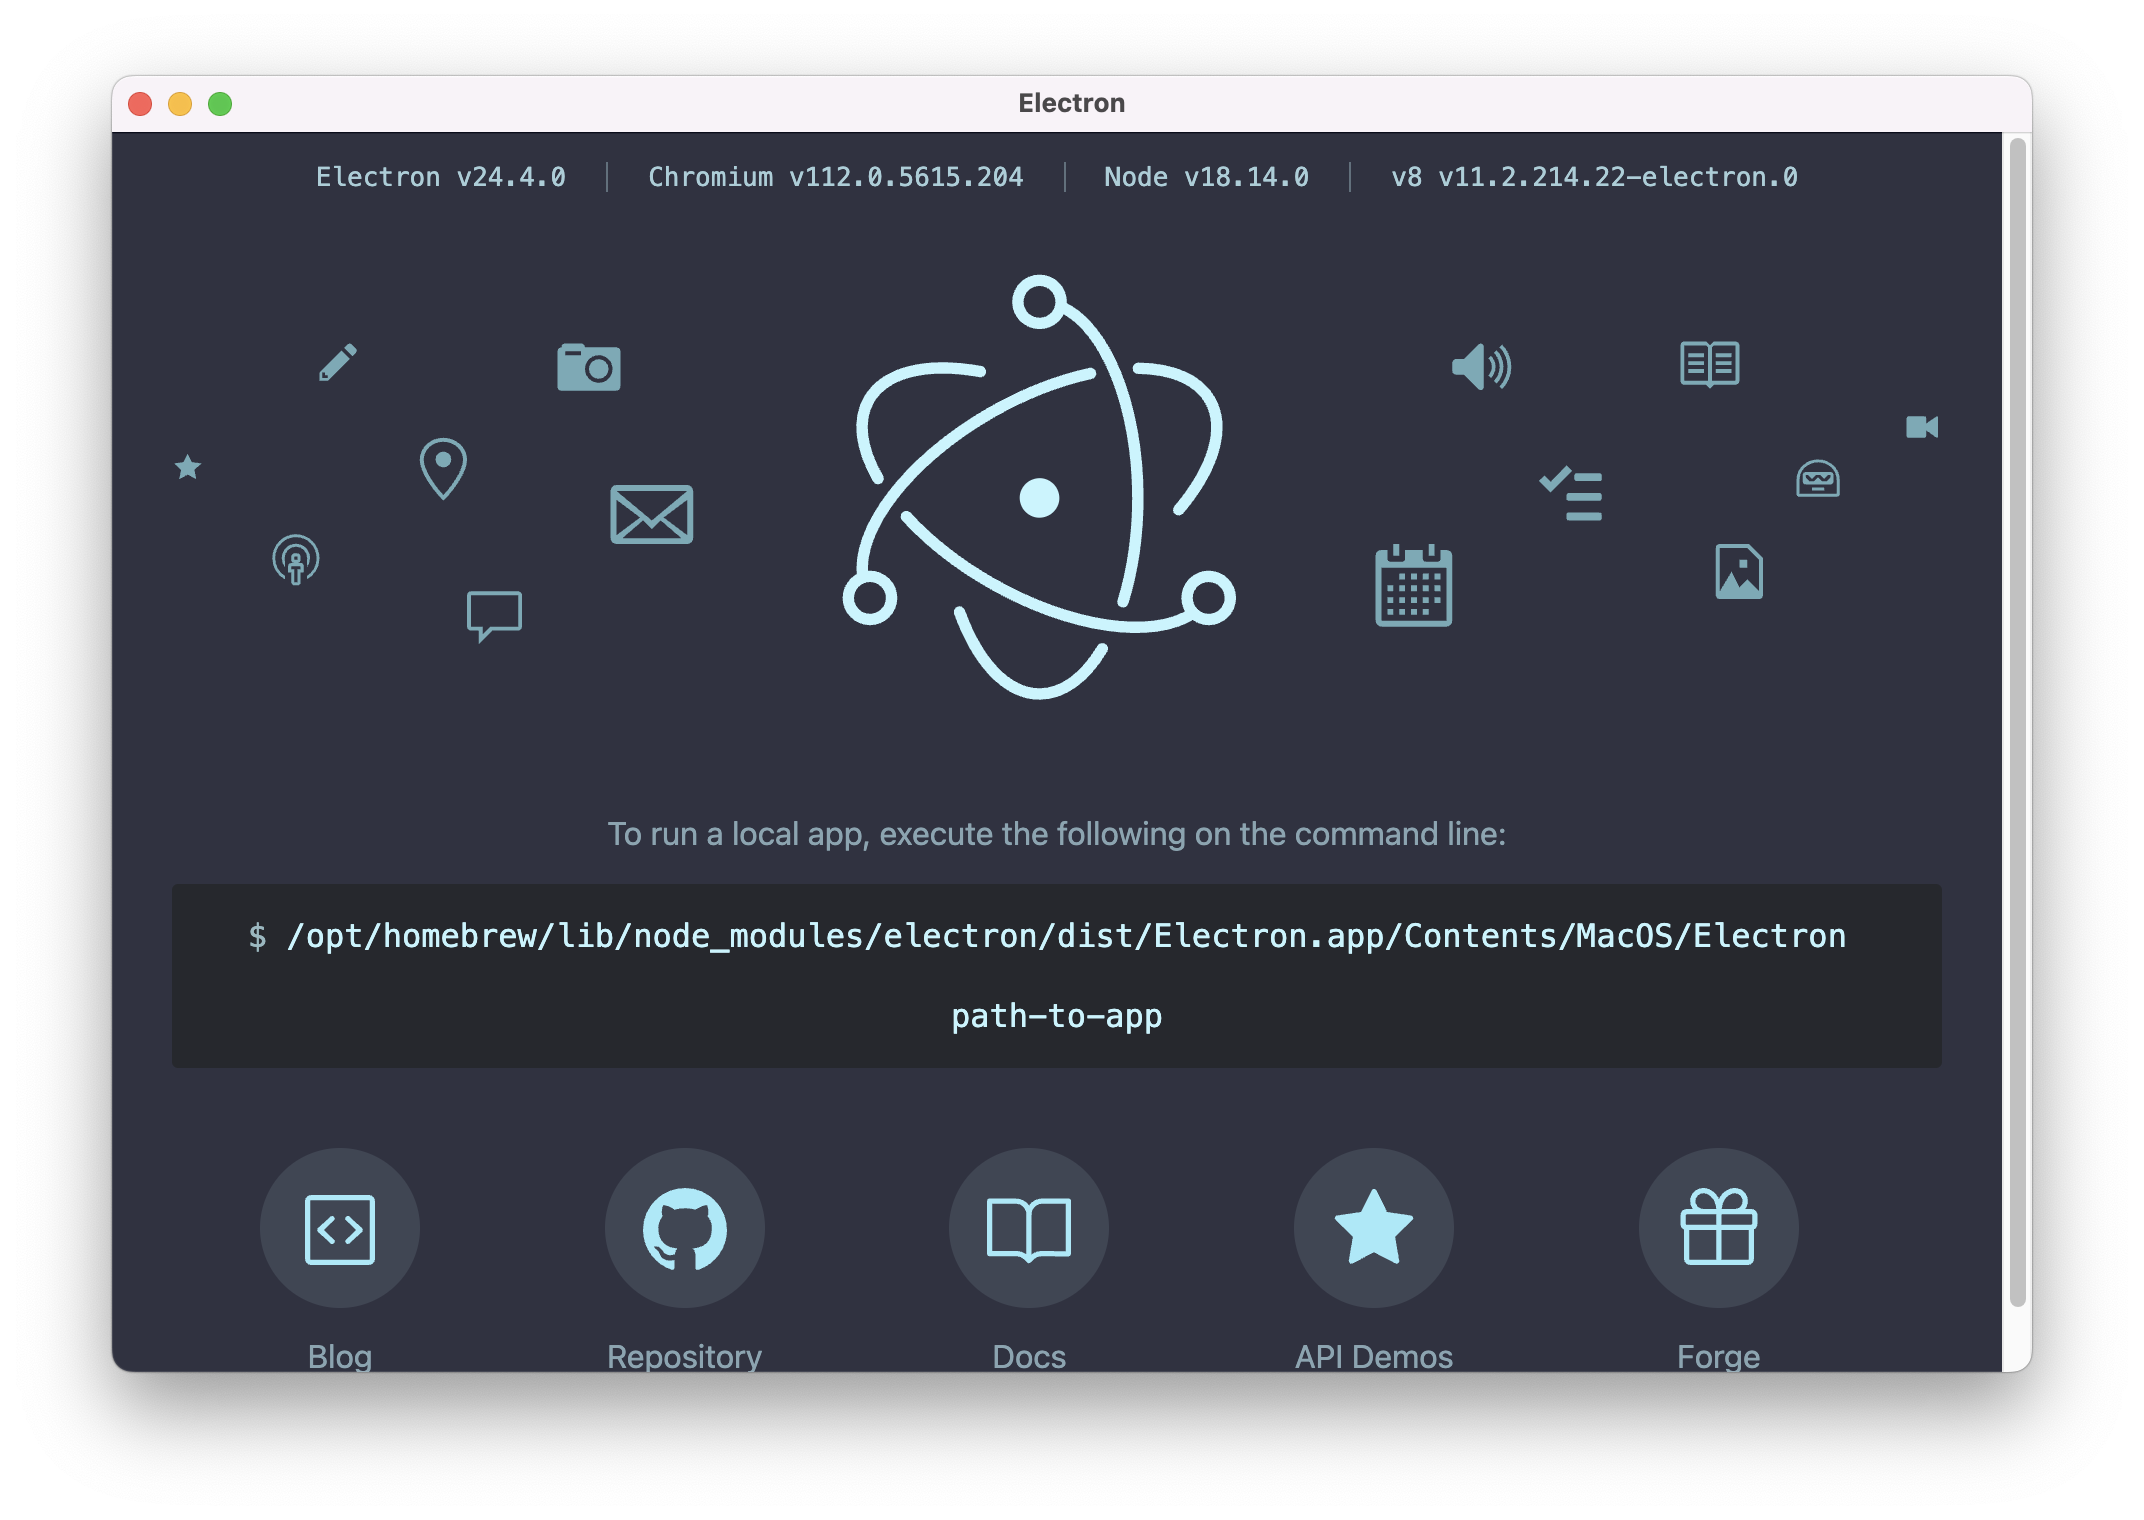
\includegraphics[width=10cm]{img/electron_default.png}

\section{やっぱり "Hello World"}
Hello Worldと表示するアプリケーションを作ってみましょう。

\subsection{作業用フォルダとパッケージファイルの作成}
今日の作業用のフォルダを「AID06」として作成しましょう。その中に「HelloWorld」というフォルダを作成しましょう。

ターミナルで\$の後に"cd "と入力した後に、作成したHelloWorldフォルダをドラッグアンドドロップしましょう。すると、
\begin{quote}
cd /Users/sammy/Desktop/AID/AID06/HelloWorld 
\end{quote}
のようになるので、リターンを押しましょう。

\begin{quote}
npm init -y
\end{quote}
とすることでpackage.jsonというファイルが作成されるはずです。VSCodeで「HelloWorld」フォルダを開きましょう。

\subsection{package.json}
アプリ作成に必要な設定ファイルです。
\begin{quote}
  "main": "index.js",
\end{quote}
と書いてある行を
\begin{quote}
  "main": "main.js",
\end{quote}
と変更しましょう。一番最初に起動するファイルが書かれています。

Electronとしては、文化的に「main.js」とするようです。次に、

\begin{verbatim}
  "scripts": {
    "test": "echo \"Error: no test specified\" && exit 1"
  },
\end{verbatim}
と書いてあるところを
\begin{verbatim}
  "scripts": {
    "test": "echo \"Error: no test specified\" && exit 1",
    "start": "electron ."
  },
\end{verbatim}
としましょう。




保存を忘れずに!

\subsection{main.js}
それでは新規ファイルでmain.jsを作成してみましょう。

\begin{lstlisting}[caption=Hello World:main.js]
const { app, BrowserWindow } = require('electron');

let win;//ウインドウを入れておく変数

function createWindow() {

    //ウインドウの作成
    win = new BrowserWindow({
        width: 400,
        height: 400,
        webPreferences: {
            nodeIntegration: true, //Electron6から必要らしい
            contextIsolation: false, //Security的には良くないらしいが...
        }
    })

    //ウインドウに表示する内容
    win.loadFile('index.html');

    //デバッグ画面表示
    // win.webContents.openDevTools();

    //このウインドウが閉じられたときの処理
    win.on('closed', () => {
        win = null;
    })
}

//アプリが初期化されたとき(起動されたとき)
app.on('ready', () => {
    createWindow();
})

//全ウインドウが閉じられたとき
app.on('window-all-closed', () => {
    if (process.platform !== 'darwin') {
        app.quit();
    }
})

//アクティブになったとき(MacだとDockがクリックされたとき)
app.on('activate', () => {
    if (win === null) {
        createWindow();
    }
})
\end{lstlisting}

%VSCodeだとElectronを認識しないので、エラーが出るようですが、放っておきましょう。
保存を忘れないくださいね。

\subsection{index.html}
17行目でウィンドウに表示する内容として「index.html」とされています。これを作成してみましょう。

\begin{lstlisting}[caption=Hello World:index.html]
<!DOCTYPE html>
<html>

<head>
    <meta charset="UTF-8">
    <title>Hello World!</title>
</head>

<body>
    <h1>Hello World!</h1>
    <p>
        We are using node
        <script>document.write(process.versions.node)</script>,
    </p>
    <p>
        Chrome
        <script>document.write(process.versions.chrome)</script>,
    </p>
    <p>
        and Electron
        <script>document.write(process.versions.electron)</script>.
    <p>
</body>

</html>
\end{lstlisting}

\begin{itemize}
\item procdess.versions.node
\end{itemize}
はNode.jsで定義されていて
\begin{itemize}
\item procdess.versions.chrome
\item procdess.versions.electron
\end{itemize}
は、Electronで拡張された機能となります。

\subsection{実行してみよう}
ターミナルで
\begin{quote}
npm start
\end{quote}
とすると、ウィンドウが次のよう表示されるはずです。(あ、この画像すでにcssついてる...気にしない...)

[注意:contextIsolation: falseのところを間違えると多分バージョン番号が出ません]

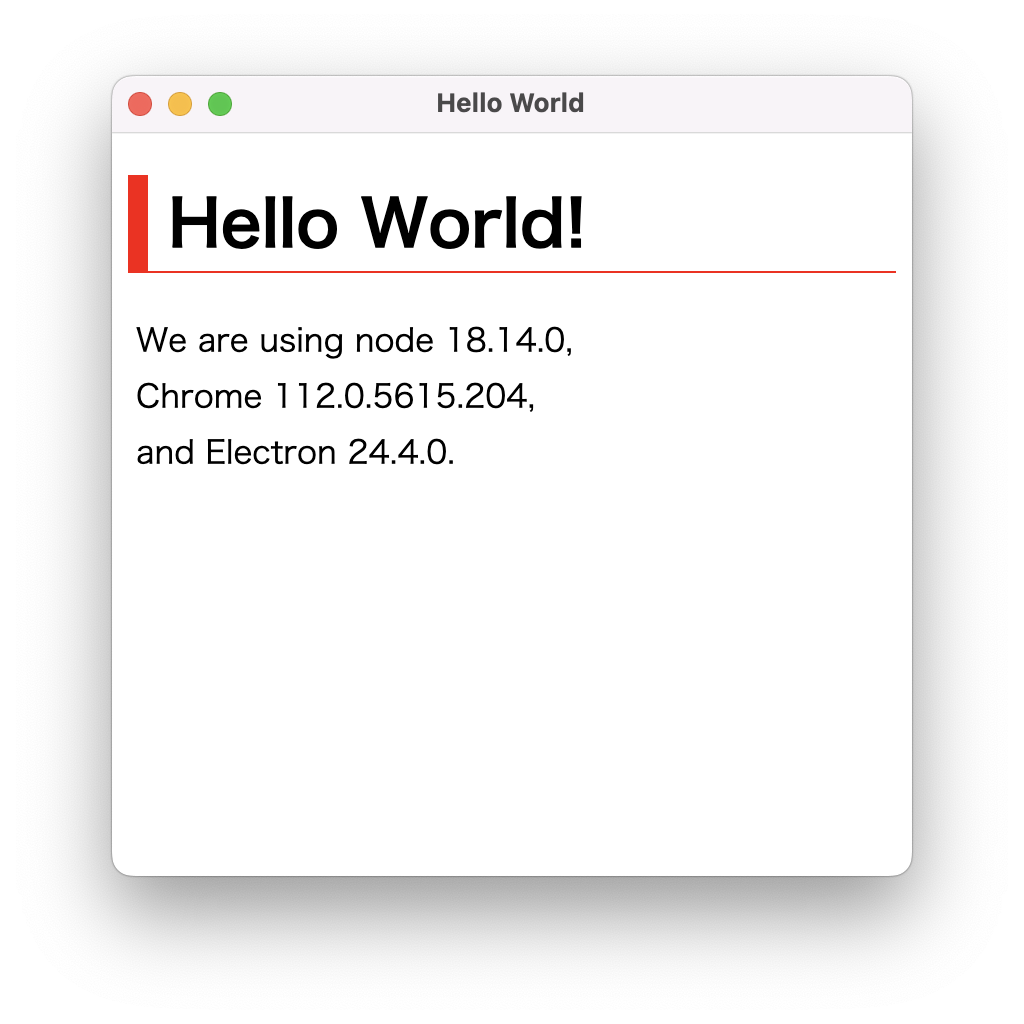
\includegraphics[width=5cm]{img/helloworld.png}

また、DockでElectronのアプリ、として起動していることも確認しましょう。

ちょっと説明します。package.jsonで
\begin{verbatim}
  "scripts": {
    "test": "echo \"Error: no test specified\" && exit 1",
    "start": "electron ."
  },
\end{verbatim}
としたため、"npm start"と入力すると、このstart部分が呼ばれて、"electron ."が実行されるわけです。

"electron ."は、このフォルダの中でelectronを実行せよ、という意味になります。

メニューから終了しましょう。

\subsection{cssを追加してみよう}
「HelloWorld」フォルダの中に「css」フォルダを作り、その中に「index.css」を作成してみましょう。

index.htmlのheadタグの中に
\begin{lstlisting}[caption=Hello World:index.html headタグ内]
    <link rel="stylesheet" type="text/css" href="css/index.css">
\end{lstlisting}
を追加して、読みに行くようにしましょう。そして、index.cssを適当に入力しましょう。
\begin{lstlisting}[caption=Hello World:css/index.css]
h1 {
    border-left: 10px solid red;
    border-bottom: 1px solid red;
    padding-left: 10px;
}
p {
    margin: 4px;
}
\end{lstlisting}
もう一度ターミナルで「npm start」で実行してみましょう。反映されてますね。Webと変わらずCSSファイルも利用することができることがわかりました。

ついでにOption+Command+Iをすると、デベロッパーツールが使えることがわかります。Webkitの技術を使っているため、ほとんどブラウザと同じ、ということになります。

Command-Qで終了できますが、ターミナルに\$マークが見えてない場合には、きちんと終了できていないため、Ctrl-Cで終了することを覚えましょう。

\section{時計作るぞ!}
%https://qiita.com/SallyAcolyte/items/94ed26ab62b8b32b1b2c

\subsection{作業用フォルダとパッケージファイルの作成}
「AID06」の中に「DigitalClock」というフォルダを作成しましょう。

ターミナルで\$の後に"cd "と入力した後に、作成したDigitalClockフォルダをドラッグアンドドロップしましょう。すると、
\begin{quote}
cd /Users/sammy/Desktop/AID/AID06/DigitalClock 
\end{quote}
のようになるので、リターンを押しましょう。

\begin{quote}
npm init -y
\end{quote}
とすることでpackage.jsonというファイルが作成されるはずです。VSCodeで「DigitalClock」フォルダを開きましょう。

\subsection{package.json}
アプリ作成に必要な設定ファイルです。
\begin{quote}
  "main": "index.js",
\end{quote}
と書いてある行を
\begin{quote}
  "main": "main.js",
\end{quote}
と変更しましょう。一番最初に起動するファイルが書かれています。

Electronとしては、文化的に「main.js」とするようです。次に、

\begin{verbatim}
  "scripts": {
    "test": "echo \"Error: no test specified\" && exit 1"
  },
\end{verbatim}
と書いてあるところを
\begin{verbatim}
  "scripts": {
    "test": "echo \"Error: no test specified\" && exit 1",
    "start": "electron ."
  },
\end{verbatim}
としましょう。

保存を忘れずに!

\subsection{main.js}
HelloWorldのものをそのまま複製しましょう。

\begin{verbatim}
        width: 400,
        height: 400,
\end{verbatim}
を
\begin{verbatim}
        width: 200,
        height: 100,
\end{verbatim}
に変更しておきましょう。
\subsection{index.html}
新規ファイルとして作成しましょう。
\begin{lstlisting}[caption=DigitalClock:index.html]
<!DOCTYPE html>
<html>
    <head>
        <meta charset="utf-8">
        <title>clock</title>
    </head>
    <body>
        <div id="digital_clock"><!-- ここに時刻が入る --></div>
        <script src="clock.js"></script>
    </body>
</html>
\end{lstlisting}

\subsection{clock.js}
前の9行目でclock.jsが呼び出されているため、それを作成しましょう。
\begin{lstlisting}[caption=DigitalClock:clock.js]
// 時計の描画処理をスタート
clock();

function clock () {
    // 現在日時を取得
    let d = new Date();

    // デジタル時計を更新
    updateDigitalClock(d);

    // 次の「0ミリ秒」に実行されるよう、次の描画処理を予約
    let delay = 1000 - new Date().getMilliseconds();
    setTimeout(clock, delay);
}

function updateDigitalClock (d) {
    const AA_str = ["Sun", "Mon", "Tue", "Wed", "Thu", "Fri", "Sat"];
    let YY = d.getFullYear().toString().slice(-2);
    let MM = d.getMonth() + 1;
    let DD = d.getDate();
    let AA = d.getDay();
    let hh = d.getHours();
    let mm = d.getMinutes();
    let ss = d.getSeconds();

    // 桁あわせ
    if(MM < 10) { MM = "0" + MM; }
    if(DD < 10) { DD = "0" + DD; }
    if(hh < 10) { hh = "0" + hh; }
    if(mm < 10) { mm = "0" + mm; }
    if(ss < 10) { ss = "0" + ss; }

    let text = YY + '/' + MM + '/' + DD + ' (' + AA_str[AA] + ')<br>' + hh + ':' + mm + ':' + ss;
    document.getElementById("digital_clock").innerHTML = text;
}
\end{lstlisting}

「npm start」でとりあえず、時計が動いていることがわかると思います。

\subsection{透過ウィンドウへの変更}
main.jsのwin=new BrowserWindow部分を以下のように3行追記しましょう。

\begin{lstlisting}[caption=DigitalClock:main.js ]
    win = new BrowserWindow({
        width: 200,
        height: 100,
        transparent: true, // ウィンドウの背景を透過
        frame: false, // 枠の無いウィンドウ
        resizable: false, // ウィンドウのリサイズを禁止
        webPreferences: {
            nodeIntegration: true, //Electron6から必要らしい
            contextIsolation: false, //Security的には良くないらしいが...
        }
    })
\end{lstlisting}

\subsection{css/clock.cssの追加}
このままだと、ドラッグも何もできないため、背景をCSSでいじりましょう。
cssフォルダを作成してその中にclock.cssを追加します。

index.htmlでcss/clock.cssのリンク追加を忘れないように!

\begin{lstlisting}[caption=DigitalClock:css/clock.css ]
body {
    background-color: rgba(24, 24, 24, .7);
    color: #fff;
    -webkit-app-region: drag;
    -webkit-user-select: none;
    user-select: none; //なくても動きますが、ないとVSCが警告を出します
}
\end{lstlisting}

ちょっと説明します。
\begin{description}
\item[背景色/背景画像]
透過ウィンドウでは「何もない部分」はクリック出来ないため、背景を指定します
rgba(r, g, b, a)による色指定を行うことで、透明度を持った背景色が指定できます
\item[-webkit-app-region: drag;]
要素をウィンドウのタイトルバーのように扱う指定です
いずれかの要素にこの指定を行わないと、ドラッグによるウィンドウ移動が出来ません
\item[-webkit-app-region: no-drag;]
dragを指定した要素内にボタンなど操作可能な要素を配置する場合、no-dragを指定して上書きします
\item[-webkit-user-select: none;]
テキストの選択を無効化します
主にインタフェース部分に指定します
\end{description}

-webkit-となっているのは「ベンダープレフィックス」と言って、Webkitのみで利用できるCSSとなっています。

index.htmlからcssファイルへのリンクを忘れないようにしましょう。
\subsection{cssの調整}
見た目をさらに調整するために、以下のようにしましょう。
\begin{lstlisting}[caption=DigitalClock:css/clock.css ]
@import url(http://fonts.googleapis.com/css?family=Iceland);

body {
    overflow: hidden;
    margin: 0;
    padding: 0;
    border: 5px solid rgb(42, 42, 42);
    background-color: rgba(24, 24, 24, .7);
    box-shadow: 0 0 8px 3px #000 inset;

    -webkit-app-region: drag;
    -webkit-user-select: none;
    user-select: none; //なくても動きますが、ないとVSCが警告を出します
}

#digital_clock {
    font-family: "Iceland";
    font-size: 25px;
    line-height: 40px;
    margin-top: 9px;
    text-align: center;
    color: #fff;
    text-shadow: 1px 1px 3px #000;
}
\end{lstlisting}

@import文は、Google Fontsというサービスを利用して、フォントを利用できるようにしています。

詳しくは
\begin{quote}
https://saruwakakun.com/html-css/basic/google-fonts
https://peraichi.com/univ/20220502
\end{quote}
をみましょう。

\section{アプリケーションとして配布できるようにしよう}
\subsection{これまで}
ターミナルで「 npm start」で起動してるので、アプリケーションっぽいんだけど、アプリケーションっぽくないですね。配布できるようにしましょう。

\subsection{electron-builder}
ターミナルで
\begin{quote}
npm install -D electron-builder
\end{quote}
としてください。1分くらいかかりますが、「node\_modules」というフォルダが増えましたね。

後、アプリ作るのに、node\_modulesの中に必要っぽいので
\begin{quote}
npm install -D electron
\end{quote}
もしましょう。

\subsection{package.json}
\begin{verbatim}
  "devDependencies": {
    "electron": "^33.0.1",
    "electron-builder": "^25.1.8"
  }
\end{verbatim}
の後に以下のように6行追記してください。「,」を忘れずに
\begin{verbatim}
  "devDependencies": {
    "electron": "^33.0.1",
    "electron-builder": "^25.1.8"
  },
  "build": {
    "appId": "jp.test.app1",
    "mac": {
      "target": "dmg"
    }
  }
\end{verbatim}

\subsection{build}
実際にファイルを構築することをビルド、と言います。

ターミナルで
\begin{verbatim}
./node_modules/.bin/electron-builder --mac --universal
\end{verbatim}
としましょう。うまくいけば、distフォルダができて、その中に配布用のdmgファイルができるはずです。

macにはIntel, AppleSiliconの二つの種類のCPUがありますが、そのどちらでも動くアプリケーションを作成するために「--universal」としています。

windowsの場合には次を参考にしてください。(うまく行くかな...)
\begin{quote}
https://maku.blog/p/2tcs8n2/
\end{quote}

\subsection{セキュリティについて}
アプリ開発時にはセキュリティについて考慮する必要があります。今回のサンプルでは煩雑になるため手抜きしています。
詳しくは次を参考にしてください。
\begin{quote}
https://gist.github.com/umamichi/5d52367235c98425e9d3fa4439d35046\\
https://zenn.dev/sprout2000/books/6f6a0bf2fd301c/viewer/13340
\end{quote}

\section{まとめ}
これまで学んできた、Canvas,WebGLもJavaScriptなわけですから、Electronを利用することでアプリケーションを開発することができたのが理解できたでしょうか?

\vspace{1em}
アイコンを変更したり、メニューバーを改造したり、普通のアプリ開発で必要なことは相当できるみたいです。

興味を持った人は、以下をみてみましょう。

https://qiita.com/nyanchu/items/9a1c910bbca55e9d2f3c

また、アナログ時計を作ってみたい人は、以下のページを見てみてください。

https://qiita.com/Yuta\_spade/items/2493c05cd868ea5f2677

\section*{P.S.}
バージョンアップすると、動かなくなるから、それの対処方法に少しハマったー


\flushright{以上}


\end{document}